%
% practice.tex
%

\section{Practice}

\subsection{Power Spectrum}
To be honest I'm not quite sure what the power spectrum describes, but it must
have to do with frequency of sorts, since it is based on a transform in that
domain. I would guess that the 2-dimensional representation thereof shows the
frequency variance within the image.

\begin{figure}[H]
    \center
    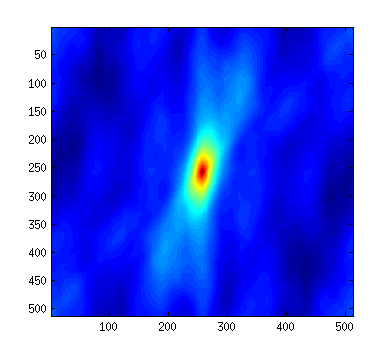
\includegraphics[scale=0.75]{figures/2-a}
    \caption{Comparison of convolution methods}
    \label{fig:2-a}
\end{figure}

\subsection{Spatial Representation}
The time required to compute the result using the fast fourier transform
convolution method (~0.05 secs) was by far faster than the for-loop method
(~2.5 secs).

\begin{figure}[H]
    \center
    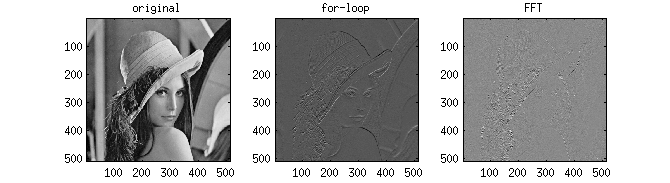
\includegraphics[scale=0.75]{figures/2-b}
    \caption{Comparison of convolution methods}
    \label{fig:2-b}
\end{figure}

As apparent from figure (\ref{fig:2-b}) above, however, the results were
nothing alike. Since the for-loop method produced what I would have expected,
this lead me to think I have a problem with the FFT convolution
implementation \ref{appendix:2-b}.

\subsection{Planar Wave Filter}
I'm not entirely sure how a filter could ever remove noise that is dependent
on the $x$ and $y$ coordinates. If my understanding of the question is correct
I would argue that since the noise introduced is structural in nature, so
must such a filter be, and thus a kernel will not suffice. We can, however,
remove the noise using an inverse operation on the image (see appendix
\ref{appendix:2-c}).

\begin{figure}[H]
    \center
    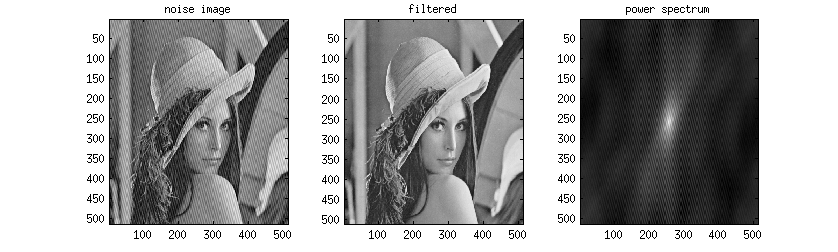
\includegraphics[scale=0.5]{figures/2-c}
    \caption{Results from wave filtering, and power spectrum}
    \label{fig:2-c}
\end{figure}

On the left we have the image with noise added, in middle we have the filtered
image, and on the right the power spectrum of the unfiltered image.

\subsection{Isotropic Gaussian kernel}
The assignment text for this task was very ambiguous, so I've done something
along the lines of what is asked, but I'm not entirely sure if it is what was
meant to be done. I've used the FFT techniques offered in the book to make a
function which basically wraps the gaussian filter in a function.

\begin{figure}[H]
    \center
    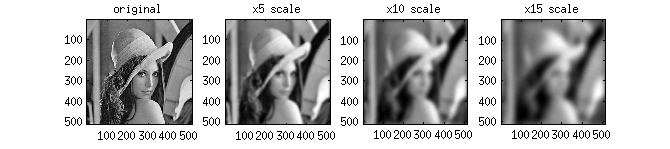
\includegraphics[scale=0.75]{figures/2-d}
    \caption{Different scales applied to an image}
    \label{fig:2-d}
\end{figure}

\subsection{Spatial Derivatives}
I didn't have time for this one :(

\subsection{Derivative Orders}
I didn't have time for this one :(
